\documentclass[oneside,11pt]{memoir}
\setsecnumdepth{subsection}
\setcounter{tocdepth}{3}


\usepackage[T1]{fontenc}
\usepackage[margin=1.5in]{geometry}
\usepackage{soul}
% \usepackage[small,compact]{titlesec} %very powerful
\usepackage[most]{tcolorbox}
\usepackage{enumitem}
\usepackage{epigraph}
\usepackage{cite}
\usepackage{caption}
\captionsetup{font=small}
\usepackage{graphicx}
\usepackage{hyperref}
\usepackage{wrapfig}
\setlength\intextsep{0pt} % remove extra space above and below in-line float
\usepackage{xcolor}
\usepackage{hyperref}
\hypersetup{
  colorlinks,
  citecolor=black,
  filecolor=black,
  linkcolor=blue,
  urlcolor=blue,
}
\usepackage{booktabs}

% \newtcolorbox{cbox}[1][]
% {
% left=1pt,right=1pt,top=1pt,bottom=1pt,
% colback=gray!10,
% boxrule=0.5pt
% }

\newtcolorbox{mybox}{
  enhanced,
  boxrule=0pt,frame hidden,
  borderline west={2pt}{0pt}{green!75!black},
  colback=green!10!white,
  sharp corners
}


\newenvironment{commentbox}[1][]{
  \small
  \begin{mybox}
    {\small \textbf{#1}}
  }{
  \end{mybox}
}


\newtcolorbox{mydomesticbox}{
  enhanced,
  boxrule=0pt,frame hidden,
  borderline west={2pt}{0pt}{red!75!black},
  colback=blue!10!white,
  sharp corners
}

\newenvironment{domesticbox}[1][]{
  \small
  \begin{mydomesticbox}
    {\small \textbf{#1}}
  }{
  \end{mydomesticbox}
}

\renewcommand{\figurename}{Fig.}
\renewcommand{\tablename}{Tab.}
\def\Section{\S}
\newcommand{\mycomment}[3][\color{blue}]{{#1{{#2}: {#3}}}}
\newcommand{\tvn}[1]{\mycomment{TVN}{#1}}{}
\newcommand{\didi}[1]{\mycomment{Didier}{#1}}{}
\newcommand{\tl}[1]{\mycomment{ThanhLe}{#1}}{}
\newcommand{\red}[1]{{\color{red}{#1}}}
\newcommand{\xz}[1]{\mycomment{Xiaokuan}{[#1]}}{}


\title{Demystifying the Computer Science PhD Admission in the US\\{\large A Guide for International Students}}

\author{\href{https://nguyenthanhvuh.github.io}{ThanhVu (Vu) Nguyen}\\{\small George Mason University, Dept. of Computer Science}}

\chapterstyle{pedersen}


\makeatletter
\def\maketitle{%
  \null
  \thispagestyle{empty}%
  \vfill
  \begin{center}\leavevmode
    \normalfont
    {\LARGE\raggedright \textbf{\@title}\par}%
    \vfill%
    % \hrulefill\par
    {\Large \@author\par}%
    \vfill%
    {\large\raggedleft \@date\par}%
  \end{center}%
  \vfill
  \null
  \cleardoublepage
}
\makeatother
% \author{ThanhVu H. Nguyen}
% \title{TITLE OF BOOK}
% \date{}


\begin{document}
\maketitle
\frontmatter

\chapter{Preface}
Having been involved in PhD admissions for many years, I've
realized that many \textbf{international students}, especially those in  smaller countries or less well-known universities, lack a clear understanding of
the Computer Science PhD admission process at US universities. This confusion not only
discourages students from applying but also creates the perception that
getting admitted to a CS PhD program in the US is difficult compared to other countries.

% though \emph{very} top schools could be very selective, e.g., see the \href{https://da-data.blogspot.com/2015/03/reflecting-on-cs-graduate-admissions.html}{admission process} at CMU
So I want to share some details about the PhD admission process and advice for those who are interested in applying for a \textbf{PhD in Computer Science in the US}.
While this document is primarily intended for students interested in CS, it may be relevant to students from various disciplines. 
Furthermore, although many examples are specifics for schools that I and other contributors of this document know about, the information should be generalizable to other R1\footnote{An \href{https://en.wikipedia.org/wiki/List_of_research_universities_in_the_United_States}{R1 institution} in the US is a research-intensive university with a high level of research activity across various disciplines. Currently, 146 (out of 4000) universities are classified as R1.} institutions in the US (and also likely universities in other countries).

In addition, this document can help \textbf{US faculty and admission committee} gain a better understanding of international students and their cultural differences.  By recognizing and leveraging these differences, CS programs in the US can attract larger and more competitive application pools from international students.

I wish you the best of luck. And if you follow this guidance, you will at least have a good chance at GMU (see
\href{https://github.com/dynaroars/dynaroars.github.io/wiki/About-GMU}{why
  you want to study at here}). Happy school hunting!

The latest version of this document is at \url{nguyenthanhvuh.github.io/phd-cs-us/demystify.pdf} and its \LaTeX{} source is on \href{https://github.com/nguyenthanhvuh/phd-cs-us}{Github}. If you have questions or comments, feel free to create a \href{https://github.com/nguyenthanhvuh/phd-cs-us/issues}{GitHub issue} for discussion.

\newpage
\tableofcontents*

\chapter{Summary}\label{sec:summary}

Here, we outline the main points of the document. This gives you an overview to decide which specific topics you want to explore more thoroughly.


\begin{enumerate}
  \item Should you apply to a CS PhD in the US?
        \begin{itemize}
          \item \emph{Yes, definitely}.  CS PhD study in the US is fully funded and admission into good universities is not any harder than non-US schools (\S\ref{sec:should}).
        \end{itemize}
  \item How is your application evaluated?
        \begin{itemize}
          \item Applications are evaluated by the \emph{PhD Admission} committee and each application is reviewed by typically 3 faculty (\S\ref{sec:evalapps}).
          \item Individually faculty \emph{cannot directly admit} a student---so do not email and ask if you have a chance. However, faculty can \emph{advocate} for a student and therefore increase their admission chance---so contact and introduce yourself (\S\ref{sec:contact}).
        \end{itemize}
  \item Application Materials
        \begin{itemize}
          \item The committee will look at various factors, but the most important ones are research ability, e.g., publications, personal statement, and recommendation letters.
          \item LORs are very important, but only if they are personalized and talk about your research ability (\S\ref{sec:lor}).
          \item Personal statement is very important. Write it in such a way that makes you \emph{stand out} (\S\ref{sec:research-statement} and \S\ref{sec:improve-your-chance})
          \item GRE \emph{is not} required (\S\ref{sec:grades}). Spend your time on something else.
          \item Grades are important, but depend on the reputation of your school (\S\ref{sec:grades}).
          \item Getting an interview is typically a \emph{good sign} (no one interviews weak candidates).
        \end{itemize}
  \item What to do after getting admitted?
        \begin{itemize}
          \item Attend \emph{Open House} to learn more about the place and \emph{interview} profs---they would be much more willing to talk to you now (\S\ref{sec:accepted}).
        \end{itemize}
  \item Funding
        \begin{itemize}
          \item TA and RA are two main sources of funding.  TA (teaching assistantship) is provided by the department to help profs. with classes (e.g., grading). RA (research assistantship) is provided by profs. to help them with their research (\S\ref{sec:funding}).
        \end{itemize}
  \item Choosing School and Professors
        \begin{itemize}
          \item Many schools do not offer PhD studies in CS and many CS professors \emph{cannot} be adviser, i.e., cannot graduate PhD students  (\S\ref{sec:schoolsandprofs}).
          \item Contacting a prof. for research opportunities is recommended, but do it \emph{properly} (\S\ref{sec:contact}).
        \end{itemize}
  \item Miscs and FAQS
        \begin{itemize}
          \item Increasing your admission chance by being unique and standing out (\S\ref{sec:improve-your-chance}).
          \item You can successfully apply to CS PhD even if you have non-STEM background (\S\ref{sec:non-stem}).
          \item Compared to other countries, CS PhD in the US does not require an MS degree but has longer PhD study time (\S\ref{sec:non-us-differences}).
          \item Your PhD costs about \$400K in total, but you do not pay for it (\S\ref{sec:ra-cost}).
          \item Despite some miserable stories on social media, many PhD students have good mentors, supportive labmates, healthy working environment ... and are happy (\S\ref{sec:happy}).
        \end{itemize}
\end{enumerate}


\mainmatter
\chapter{Should You Apply to a CS PhD Program in the US?}\label{sec:should}

\epigraph{\vspace{-0.2in} Don't make fun of graduate students. They just made a terrible life choice.}{\textsc{The Simpsons}}

First, I want to emphasize that PhD students in Computer Science \emph{do not} need to worry about funding, especially at good R1
universities in the US. If you are admitted, you will almost certainly
receive \emph{full funding} to support your study, including tuition,
health insurance, and stipend (monthly salary). Moreover, depending on the university,
you may even receive additional benefits such as summer pay, laptops, (conference/workshop) traveling. \S\ref{sec:funding} provides more details on funding.

Second, applying to a good US university \emph{should not} be any harder than at schools in other countries. In fact, it might even be more flexible since CS PhD in the US \emph{do not} require having an MS (or having to know a topic/proposal/adviser in advance). If you believe you have a chance in other countries, e.g., South Korea, Singapore, Germany, UK, Japan, and Australia, then you will surely have a chance in the US as well. \S\ref{sec:non-us-differences} compares CS PhD study in the US to other countries.

\begin{commentbox}[Vu:]
  One of the reasons I create this document is that my colleagues at GMU are interested in recruiting Vietnamese students and are surprised when seeing very few applications in Vietnam (see \S\ref{sec:ack}). Each year our CS program receives more than 350 PhD applications, most of which are international but only 3--4 are from Vietnam. In general the number of CS PhD applications from Vietnam to US universities is very low and more would be welcome.
\end{commentbox}

\begin{domesticbox}[Domestic students:] If you're a domestic student, you have several advantages in your application.  First, we already know about your school (see \S\ref{sec:your-school}), and you are also more familiar with the US education system and culture.  You also have more opportunities for funding, e.g., through government scholarships for US citizens and residents. Finally, compared to international students, PhD applications in CS from domestic students are few and that can help your case.
\end{domesticbox}

%% Vu: *what's a PhD?*  This [[https://matt.might.net/articles/phd-school-in-pictures/][series of pictures]] from [[https://matt.might.net][Matt Might]] illustrates what a PhD means.
%% \end{commentbox}

\section*{References}
\begin{itemize}
    \item \href{https://parentheticallyspeaking.org/articles/us-cs-phd-faq/}{Getting a Computer Science PhD in the USA} by Shriram Krishnamurthi
\end{itemize}

\chapter{How is Your Application Evaluated?}\label{sec:evalapps}

\epigraph{How is education supposed to make me feel smarter? Besides, every time I learn something new, it pushes some of the old stuff out of my brain. Remember when I took that home wine making course, and I forgot how to drive?}{\textsc{The Simpsons}}

After you submit your PhD application (usually November--December), it will be first screened
for general requirements, e.g., did you submit your transcripts and standard scores? did your reference writers submit their letters?

Then, applications are reviewed by a \textbf{PhD admission committee} that consists of faculty members in CS (in some cases the committee can involve affiliated faculty from different disciplines). These faculty have a wide-range of expertise and background to ensure diverse perspectives in the evaluation process. The size and the review load of the committee depends on the department size. At GMU, the PhD committee typically has 15--20 faculty, and each committee member is assigned to review 25--30 applications. Note that GMU, UMass, and probably many other schools, have separate committees for MS programs.

Each application is assigned to about \emph{three} faculty members, who will evaluate your profile and reach a consensus.  Note that while the assigned reviewers are likely the main ones deciding your application, \emph{every} faculty in the department will have access to your application and can provide inputs and opinions on your profile.

The PhD admission committee typically involves assistant professors in the department (see \S\ref{sec:faculty-types} for various faculty titles). This provides junior faculty the opportunities to recruit students. The chair of the committee will be a senior professor, but they likely will not review individual applications and instead assign them to committee members. The chair will look at various factors such as research interests or mentioning faculty names to assign the applications to appropriate faculty. 

At GMU, we usually decide that a full-time PhD candidate is either (i) admit with funding (TA or RA, see \S\ref{sec:funding}) or (ii) rejected. In other words, in most cases, we either
admit you with full funding, or we reject your application. In some rare cases, we admit
without funding because you have funding on your own (e.g.,
supported by your government or having external grants). We also justify
our decision with a summary of your application, where we list
strengths (e.g., a well-known school) and weaknesses (e.g., weak
LORs). 

% \didi{Is there more information on typical strengths and common weaknesses of applications. This is especially useful to sophomore and junior students as they still have time to work on those strengths.}
% tvn: the main thing is research experiences

\begin{commentbox}[Hakan:]
  At GMU, for full consideration, students should make sure to submit \textbf{ALL} required documents by the application deadline, and should never assume that some required documents (such as official TOEFL scores or official diplomas/transcripts) will be waived by the admissions office. If something is listed and not marked as ``optional'', it is mandatory and they should plan for submitting all those.
\end{commentbox}
\paragraph{Why we do not waive application fee?}  This is typically a requirement of the university. Individual departments and programs do not have the flexibility to waive the application fee, even if they want to. 

In my opinion, requiring applicants to pay the fee helps ensure their seriousness, as it filters out non-serious candidates. Also, if the application process were free for everyone, we would receive an overwhelming number of applications to review.


% \begin{commentbox}[Hung]
%   The application fee varies between schools, and is about \$70--\$100. I found this number pretty ridiculous. In most cases, there is no proper justification for that amount. Yes, the application fee could act as a filter, but a nominal amount would do the job. While a blanket waiver might not be feasible, universities should extend the eligibility of fee waiver applications to more countries.
% \end{commentbox}


\chapter{Your Application}\label{sec:application}

\epigraph{Son, if you really want something in this life, you have to work for it. Now quiet! They’re about to announce the lottery numbers.}{\textsc{The Simpsons}}


The primary focus of the admissions committee is to \textbf{evaluate your background and interest in research} (a PhD in Computer Science is a research degree!), and determine if you would \textbf{fit into} the program. To evaluate your profile, we consider
the following key indicators.

\section{Research Ability}\label{sec:research-ability}

The most effective evidence of research ability is having \textbf{published papers in reputable international journals or conferences}.
Having papers published is a sign that the applicant has successfully involved in research.

\begin{commentbox}[Vu:]
    Many international students mention Scopus Q1, which consists of various journals from IEEE, Elsevier, and many other publishers.  I don't know/recognize many of journals listed in Scopus Q1. This might be something to be mindful of, as \textbf{CS} faculty might not be too familiar with Scopus or journals listed there, so devote some part in your statement to discuss the significance of your papers.
\end{commentbox}

However, it is understandable that many students do not have the opportunities to publish in top places. Thus, general writings, even those under submissions or rejected, would still be good (and much better than nothing).  But be sure to upload your papers with your application and talk about them in your statement (see \S\ref{sec:research-statement}).  Note that local conferences and non-English journals or conferences do
not carry as much weight since their quality is often unknown to US faculty. However, if you have published in such places, you should still mention them in your statement and explain why they are good.

% In CS, conferences are important and top conferences are prestigious. You can find top CS conferences at places such as \href{https://csrankings.org}{CSRankings}, which ranks CS programs based on how their faculty publish at top \emph{conferences} (see more in \S\ref{sec:ranking}).



\begin{commentbox}[Craig:]
  GMU and many other universities allow you to upload your published papers and other writing samples. In many cases, even if the papers were not published at top places, we can still determine their quality by simply skimming over the paper.
\end{commentbox}

Additionally, \textbf{work experiences at renowned research laboratories}, such as Microsoft Research, can significantly strengthen your
application.  Unfortunately, many good research places in your countries, e.g., VinAI in Vietnam, remain relatively unknown to most universities in the US. So you should explicit say something about them in your statement.



\begin{commentbox}[Hung:]
  The reputation of VinAI has been increasing steadily over the past few years; many of my colleagues heard about VinAI.
\end{commentbox}

Finally, \textbf{participating internationally recognized competitions} can also demonstrate your research potential.
For example, participating in Math Olympiads if you want to do theory or  winning ACM programming contests if you want to ``build'' stuff, e.g., software analysis.

\begin{commentbox}[Thanh:]
  Due to academic culture, professors in Vietnam usually aim for (international) journals instead of conferences. Could you give some tips on how to know whether a journal is good (CSrankings, unfortunately, only consider conferences)?.
  \tcblower
  Vu: One way is looking at what well-known researchers publish at. For example, if you are interested in a field X, you can use CSRankings to look at active faculty in X, and then look at their websites to see what journals they publish at.
\end{commentbox}

\section{Letter of Recommendation (LOR)}\label{sec:lor}

\begin{center}
    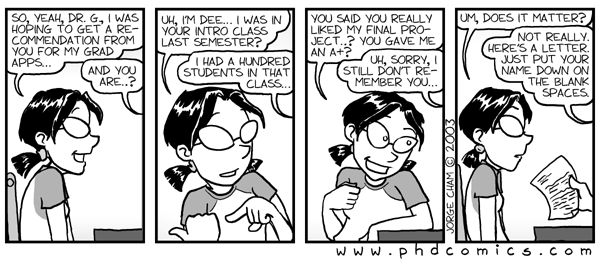
\includegraphics[width=0.6\linewidth]{files/c6.png}
  \end{center}
  

  
Most PhD programs will require at least \textbf{two LORs}. Having a letter from an internationally recognized researcher can greatly strengthen your application. However, obtaining such letters
can be challenging for international students, who might not have much interactions with such experts. So it is fine to have a letter from people (e.g., profs, researchers, postdocs who mentored you) that know you well enough to talk about \emph{your research experience and capabilities}. Many students get letters from supervisors from companies where they did internships or are working at. It is OK as long as it is a research-based personalized letter (once again, we are talking about PhD applications, not MS).



\begin{commentbox}[Vu:]
    If your grading system is not US standard or you are from a good school unknown outside of your country, you can ask your reference writers to explain about that in their letters.  For example, "Bach Khoa" are the top universities in Vietnam for STEM studies but few people outside Vietnam know about them.  So if you are from there, you should ask your reference writers to mention that.
\end{commentbox}

\paragraph{Self-written Letters} Many international students write letters themselves (typically due to the requests of their profs.) and have them signed by their profs. Such letters have little values and would be considered weak by reviewers, who can question why you cannot even find someone cares enough about you to write a candid personal reference letter.  Instead of the reference writer writing about you, in this case it is you who write about yourself (and they just sign the letter).

\paragraph{Generic Letters} When the writers do not know much about the applicants (e.g., just taking some course with them or not making any impression to write about), they might write a generic letter, which is not useful and also considered weak.  It might be a good idea to directly ask if the prof. is willing to write a \emph{strong} letter for you. If not, then you should ask someone else.  For example, if a student I don't know well ask me to write letter for them, I will explicitly tell them I don't know them that well to write much about them, and such a short, generic, and weak letter will not help their case.







\begin{commentbox}[Vu:]
  Some letter writers ask the applicants to write their own letters for them to sign. As mentioned, this will hurt the applicants (admission committee members are actually quite good at determining this)! Multiple students mentioned that  some professor did this so that the applicants do not go abroad or only go to places where they want the students to go to.
  \tcblower
  Sometimes students would go through great length just to get letters from well-known professors in their school, but the letters are generic and carry little value, in fact, \red{red flags}. Moreover, a top professor in Vietnam might not be well-known to US faculty (see more details in \S\ref{sec:your-school}). So save the trouble and just get letters from \emph{any} professors/supervisors who knows you well and can write a good letter about your research ability. It's better to have a good personalized
  letter about your own research ability from someone who is less
  well-known than a generic/weak letter from a well-known person.
\end{commentbox}

\begin{commentbox}[Hung:]
  A sad reality is that most professors in Vietnam \textbf{DO NOT} know how to write a good letter, or are lazy in writing letters hence delegate the writing to the students. Unfortunately, there is no easy solution to this problem.
\end{commentbox}

\paragraph{Waiving your Right to Review LORs}  Choosing not to look at a reference letter is pretty standard in school and job applications. When you waive your right to see the letter, it adds a layer of trust, showing you're confident in your choice of referees and that you're not trying to twist their words. It's also about keeping things open and honest between you and your letter writers, and encourages them to be real about your strengths and qualifications. Plus, it keeps things private.

Reviewers might raise concerns (a red flag) about  a letter that is not waived, e.g., if you do not trust your letter writers, then you should find someone else to write for you. In short, it's a standard practice and a way of keeping things straightforward and respectful in the whole recommendation game.

\begin{commentbox}[Didier]
  \emph{Should letter writers have PhDs?}  In Rwanda, a lot of students interact more with teaching faculty who might not have PhD.
  \tcblower
  \textbf{Vu}: This is an interesting and useful detail that US faculty might not be aware of and students should mention about this in their statements. In general, I think it should be fine as long as that person can properly evaluate your research ability.
\end{commentbox}

\paragraph{Reminding Writers to Submit Letters} After you submit your application, you can tell your writers that and remind them to submit their letters if they haven't done so. But don't send too many reminders as that can be annoying to the writers.

Note that most places only have deadlines for the applicant, but are very flexible with the letter writers (in many cases do not even give them any deadline).  Also, many places do not begin the admission review process right after the deadline and work on application reviews in the next semester (mid January).


\paragraph{VEF 2.0} For Vietnamese students, it's worth mentioning about the \href{https://vef2.org/}{VEF2.0 program}, which has helped many good students in gaining acceptance to top PhD programs in the US. VEF2.0 follows an interesting model where US faculty members from leading institutions are invited to conduct rigorous interviews with VEF students and subsequently provide reference letters on their behalf. Despite the limited interaction between the interviewer and the interviewee (primarily confined to the interview itself), these reference letters are generally helpful as they have helped many students getting into top PhD programs in the US.

\section{Statement of Purpose (SOP)}\label{sec:research-statement}

\begin{center}
  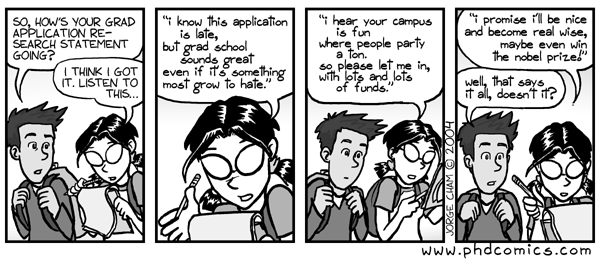
\includegraphics[scale=0.4]{files/c2.png}
\end{center}

While you might not have control over LORs or \hyperref[sec:your-school]{where your go to school}, you do over your
statement of purpose (SOP) or personal statement! So write it well because it could make a big difference.
In your statement, you have the opportunity to make your application stand out and unique, which can make you \emph{fit} the CS program you're applying to, even if you don't have very strong research experience.
A well-written LOR also shows that you can communicate, which is very important in research, and that you can effectively teach and communicate with students, which is important for TA funding (see \S\ref{sec:funding}).
% is important because if you need (GTA) funding, it will provide evidence
% that you can teach and communicate with students.

There are various guides on writing statement, e.g.,~\cite{blattman2022writing}, and \href{https://cs-sop.org/}{many example statements} are available. So I will not talk too much about statements. In short, talk about your research goal and vision, and convince us that you can achieve it through your experience, e.g., published papers, or if you work on some projects by yourself, talk about it. Also, use the statement to talk about things that admission committee members might not know about, e.g., your Github project with 1K+ stars or your regular contributions to well-known open-source projects. Finally, talk about what makes you different than the other 1000 applicants that we are considering (e.g., see \S\ref{sec:improve-your-chance} for increasing your admission chance).



\begin{commentbox}[Hung:]
  I think asking for a “research vision” from a Ph.D. applicant is too much. Even people graduated with a Ph.D. have a great difficulty in explicating their research vision. In my opinion, you should focus on showing (not telling) your research passion (if you do have).
\end{commentbox}

Finally, this is something easy to do, but is neglected by many
applicants: \textbf{customize the statement} for the school you're applying to,
e.g., why do you apply \emph{here}? provide names of professors who you're interested in (in many cases your application will be forwarded to them for evaluation).
This shows that you're serious and have done homework on places you're applying to.
Admission committee will look for this part at the end of the statement, so do not skip it.



\begin{commentbox}[Vu:]
  I often read the research statement (and the LORs) first. If I am
  persuaded by then, I would skim over other factors and advocate for
  admission (unless I see red flags in other parts). If I am not
  convinced, then I will likely recommend rejection (unless I see
  something standout in other parts).
  \tcblower
  Do careful research on professors, don't mention \emph{emeritus} or  adjunct faculty.
  Also, be careful not to send statements to wrong schools or mixing
  facts (e.g., talking about school X but mentioned about working with
  profs. at school Y; and definitely do not talk about George Washington when applying to George Mason). I have seen such statements more time that I
  should.
\end{commentbox}

\subsection*{References}
\begin{itemize}
\item \href{http://www.pl-enthusiast.net/2022/10/03/how-to-write-a-grad-school-personal-statement/}{How to Write a Grad School Personal Statement} by Mike Hicks
\end{itemize}
% \subsection{Outline of a LOR}\label{sec:lor-outline}

\section{Your School}\label{sec:your-school}

Graduating from top universities \emph{that we recognize} helps. For example, if your school is well-known, then it is \emph{``top foreign''}, which is definitely a plus.
However, if committee members do not know much about schools in your country, they will likely treat your school as
\emph{``unknown foreign''}, which can be a minus point because we are uncertain about the quality of your school.


So what can you do about this? several things including asking your CS dept to put itself on CSRankings (it's the easiest way to get CS people to know about the school and its CS faculty)  and explaining about your school in your statement (ask your LOR writer to do that too). Of course, if you're interested in working with Vietnamese, consider  \href{https://github.com/dynaroars/dynaroars.github.io/wiki/Viet-CS-Profs-US}{CS PhD programs in the US that have Vietnamese professors}.

\begin{commentbox}[Vu:]
  Sometime PhD admission committee in the US will share a document such as \href{https://github.com/dynaroars/dynaroars.github.io/wiki/Foreign-Top-Schools}{this one}, which lists the top schools in several countries. In some cases we ask other faculty and students if we think they know about the place.  For example, when I was a postdoc at UMD, people in admission committee ask me to evaluate applicants from Vietnam.  During my time at UNL and now here at GMU, I have looked at Vietnamese applications (whether they are assigned to me or not) and provide input to their reviewers, e.g., X is the top tech school in Vietnam and so it should be \emph{top} instead of \emph{unknown} foreign, which makes a huge difference.
\end{commentbox}
\begin{commentbox}[Deepak:] 
If an applicant is anxious about their school not being known outside their country, they can provide information about their school and department, with independent sources where such information can be verified.
\end{commentbox}

\section{Grades and GREs}\label{sec:grades}


Having good grades is important, but unless your school is well-known, having top grades or rankings
usually will not help because we cannot evaluate them.

This can be an issue for students in many top international universities where the competition is so high that very good students students can still have low rankings from these schools (and be overlooked by the admission committee).
So what to do with this? as mentioned in \S\ref{sec:your-school} you can put a note about this in your statement and ask your LoR writers to talk about it.

Note that while having good grades at unknown school might not help,
having very bad grades will be \red{red flag} (unless your LORs or
statement give a proper explanation). This is especially true if you
have bad grades in relevant courses (e.g., Math and CS).

\begin{commentbox}[Thanh:]
  Vietnamese universities typically offer specialized programs, such as the talented engineer program at HUST, that have highly competitive entrance exams and a limited number of available slots (e.g., 30 per year). However, these programs often set higher requirements for students, including more demanding tests and assignments, resulting in lower GPAs and overall rankings. For example, an 3.5 GPA students from such talented programs are typically much better than a 4.0 GPA students not in those programs.  Similarly, variations in GPA standards exist among different universities, with technical universities generally having lower GPAs than economical universities. These make gaining admission in the US difficult as US faculty are not familiar with these issues.
  \tcblower
  \textbf{Vu}: Vietnamese students and even faculty often lament how this grading system hurts Vietnamese students applying abroad. One way to mitigate this is making these issues known to admission committee in your statement.  Universities with Vietnamese profs are probably aware of them, but in general your letter writers \emph{and} you can explicitly mention these in their letters and your statement.
\end{commentbox}

\paragraph{GRE} Most good CS PhD programs in the US \textbf{no longer require GREs}, so you don't need to take them. However, they might be useful for international students from programs we are not familiar with.  If you have good GRE scores then you should include them in your application.

\paragraph{English Test} Unless your degrees are from specific countries such as \href{https://github.com/dynaroars/dynaroars.github.io/wiki/About-GMU#standard-tests-waiver-eligible-countries}{these}, you will need to
take standardized English test. Just do well enough to pass minimum requirement set by the university, which has many options for you to select from.

\begin{commentbox}[Vu:]
  The minimum for GMU (being above this might not mean much, but below is a \red{red flag}).
  \begin{itemize}
    \item GPA: $\ge 3.0$ in your undergrad (but we also consider the rank/prestige of your school)
    \item GRE: not required, though it can help boost your profile
    % \item but if you want to use it, then we expect a total (V+Q) of $\ge 311$ (with a $\ge 157$ Q) and A $\ge 3.0-3.5$.
    \item English requirement tests (one of the below)
          \begin{itemize}
            \item TOEF: 88 pts in total AND $\ge 20$ points in each subsection OR
            \item IELTS: $\ge 6.5$ OR
            \item DuoLingo Graduate English: $\ge 120$ OR
            \item Pearson Test of Academic English: $\ge 67$
          \end{itemize}
  \end{itemize}
\end{commentbox}


\section{CV/Resume}
The CV/Resume should provide a summary of the applicant's achievements.  It should allow the reviewers to quickly scan to identify standout achievements (e.g., Publications, Programming Competition Awards, Teaching Experience).

\section{Interview}
Sometimes a faculty wants to interview an applicant to make a decision. Typically, this means that they are considering admitting you. If they are not interested in your application, they will not proceed with an interview. 

Typically, an interview takes about 15-30 minutes, and one important aspect of evaluation is your ability to effectively communicate, including speaking and understanding English. In addition, during the interview, you will have the opportunity to ask questions about the university. It's essential to prepare some thoughtful questions, similar to a job interview.


\begin{commentbox}[Vu:]
  At GMU, we are encouraged to interview candidates. For very strong candidates, the interview is actually to recruit them.  In some cases a faculty interviews a candidate that they see potentials and want to advocate for their admission. Without the interview, such applications may be more likely to be rejected. Overall, being selected for interview means a very good chance of being admitted.
\end{commentbox}


\section{Preparing Materials}
\subsection{Sharing spreadsheets}
Many students use a spreadsheet to help them and their letter writers to keep track of their applications. You can create a personal and a shared spreadsheet but a simplest one is just a shared one (e.g., using Google sheet).  Here are some information to put on the sheet.  
\begin{itemize}
\item \textbf{Your info}: Full name, email, phone, link to website/CV).  This is helpful for the writers just in case they want to quickly get some information about you.
\item \textbf{Applications details}: University, Dept, Application System URL, Submission Deadlines, Application Status (e.g., submitted,  rejected, wait-listed, accepted)
\item \textbf{LoRs}: Writer 1, Writer 2, Writer 3.  If this is a shared document, you might want to omit names and just use writer X. Under each is their status, e.g., sent/not yet/reminder needed, etc.
\end{itemize}

\chapter{Getting Admitted}\label{sec:accepted}

\epigraph{"Oh... and how is education supposed to make me feel smarter? Besides, every time I learn something new, it pushes some old stuff out of my brain. Remember when I took that home wine-making course and I forgot how to drive?"}{\textsc{The Simpsons}}

By around March you should hear back from most PhD programs you applied to. If you haven't heard back, reach out via email and ask about the status of your application.
If you receive offers, congratulations!  Now you're at a different game because the schools that have admitted you will try to get you to accept them!  Important factors to consider are the reputation of schools and professors (\S\ref{sec:schoolsandprofs}), and of course, funding availability (\S\ref{sec:funding}). You will have to make your decision by around \emph{April 15}.

\paragraph{Open House} Most schools will have \textbf{Open House} events, which are a great resource to learn about the school, department, faculty, research, living, etc. Even if you can't come in person, you still can attend virtually and meet with individual faculty.
During the Open House, you get a chance to talk to individual faculty and current students.  Take notes of faculty who make you excited, count those that are taking in new students (if they meet you, likely they are considering new students!).  Talk to students about their advisers, the dept, the area, funding situation etc.  Ask about anything you want to determine that they deserve \emph{you}.

\begin{commentbox}[Vu:]
  GMU has \emph{Virtual} Open House (VOH), e.g., \url{https://cs-gmu.github.io/cs-phd-voh-s23/}. We invite all admitted PhD students to the VOH through Zoom to learn about the CS program, the department, GMU, and the DC area in general. Students also get opportunities to chat with professors and current students.
\end{commentbox}

\paragraph{If you do not get admitted} If you do not get admitted to any schools (or don't want to go to the ones that admit you), try again next time.  Graduate admission can involve randomness and noise.  Don't bother asking for feedback, you will not likely get any.  In the meantime, you can work on improving your profile, e.g., get more research experiences, publish more papers, improve your connections for better LoR writers, etc.

You can also consider applying to MS programs, which are typically easier to get in (but you need to pay).  If you get in an MS program at a school of your choice, you can contact professors to work with them. If you do well, you can ask the professor to support you to convert to PhD.  This is a common path for many students.


\chapter{Funding}\label{sec:funding}

\epigraph{Bart, with \$10,000, we’d be millionaires! We could buy all kinds of useful things like…love!’}{\textsc{The Simpsons}}

As mentioned, if you're admitted to a \emph{good} CS PhD program, you should not have to worry about funding!  
In the US, the common types of funding for PhD are \emph{graduate teaching assistant} (GTA or TA), \emph{graduate research assistant} (GRA or RA), and \emph{Fellowship}.
RA is paid by a prof. for you to do their research. TA is paid by the department for you to help with teaching. Finally, fellowship is an independent funding that can come from a school, a company, or an organization. Tab.~\ref{tab:funding} summarizes the differences.
Note that funding is typically more available for PhD students than 
Masters. %Undergraduates typically have no funding and also have to pay international tuition, which is very expensive!.  

\begin{table}
  \centering
  \footnotesize
  \caption{Different types of PhD funding. All Covered: includes tuition, insurance, and stipend.}\label{tab:funding}
  \begin{tabular}{c|c|c|c}
    \toprule
    &\textbf{TA}&\textbf{RA}&\textbf{Fellowship}\\
    \midrule
    \textbf{From} & School & Profs. & School/External\\
    \textbf{For}                  & Teaching Assist.       & Research                        & Research                              \\
    \textbf{Cover All?} & Yes                      & Yes                             & Yes                                   \\
    \textbf{Summer?}              & No                       & Maybe                           & Yes                                   \\
    \midrule
    \textbf{Pros}                 & Research Freedom         & Get to do research              & Research Freedom                      \\
    \textbf{Cons}                 & Teaching Duties           & Research Restriction & Competitive, Limited             \\
    \bottomrule
  \end{tabular}
\end{table}

\section{Graduate Assistantship (TA/RA)}
The most common type of funding is \textbf{graduate assistantship}, which is either TA or RA. Both TA and RA come with tuition waiving (you don't have to pay tuition), health insurance (this takes care of your insurance, which is a must have in the US), and most importantly, your stipend (i.e., your salary). Some universities also pay insurance for spouse/children (or give very good discount).

Several things about stipends.  First, the amount of stipend depends on the university, which in turn depends on various factors such as location (e.g., a stipend in Washington DC is likely higher than in Lincoln, Nebraska due to higher living cost). Second, a school year is typically 9-month in the US, so stipend is for 9 months (so divide by 9 for each month). Third, like most source of income in the US, you will have to pay tax on your stipend.  Fourth, CS department typically has higher stipend comparing to other study fields.  Finally, private universities might pay more for stipend (but they could have higher "activity" or some other hidden fee, or you may be required to pay fees for each credit hour).

Students often complain their stipend being too low, but it is actually not bad and you can live comfortably with it.  In many cases, it is also enough to support your spouse and kids (many CS PhD students have their family with them). So don't worry too much about stipend.  If you're admitted to a good CS PhD program, you will be fine. A good school would know that it has to be competitive to attract students.  For example, at GMU, every year we discuss about improving the benefits, and especially stipend, for our graduate students. 

For a full breakdown of how much a graduate student costs, see \S\ref{sec:ra-cost}.

\begin{commentbox}[Vu:]
  TA and RA at GMU have similar benefits in tuition waiving and insurance.  The college and department will set the rate for 9-month graduate assistant stipend.  TA, which is paid by the department, will likely be that amount but RA might be higher depending on the stage of the student (1st year vs ABD\footnote{All but dissertation: really close to graduate.}) and the prof.
  \tcblower
  Having health insurance is required at many US universities.  Do not assume that you're young and healthy and ignore insurance.  At GMU, and at most good CS PhD programs, your GTA or GRA \emph{will always} come with full insurance. In fact, at GMU your spouse/children will get significant discount rate for health insurance.  So you will never have to worry much about health issues for you or your family here.
\end{commentbox}


\subsection{Teaching Assistant (TA)}\label{sec:ta}

TA is common in the beginning when you haven't found an adviser who would pay you RA. As a TA, you spend up to 20 hrs/week and help with classes (e.g., grading or teaching labs/recitation). Your TA is paid through the school or department, i.e., they hire you to help teach.  During a semester, a TA might work with several courses and professors (not necessary their adviser).  TA funding is not typically available during the summer, which has few courses.

\paragraph{How to get TA?}  Unless you have other funding such as RA or Fellowships, TA is typically default for good CS PhD programs. When you apply to be a full-time student,  state that you need financial assistant. It is common that the PhD committee will either admit you and give you GTA, or reject you; i.e., we do not admit a student without supporting them.  

\begin{commentbox}[Vu:]
  At GMU CS, students admitted with TA have  4 years of GTA guaranteed, and in some cases also receive  stipend for the first summer.
\end{commentbox}

Even if you have other funding and do not need TA, you still should do TA at least once.  This allows you to see what teaching is like, which is especially helpful for research career where you often give talks and tell people about your work. GMU sometimes has classes that a more senior student can teach.  In that case, you will be paid as GTA or even sometimes as a lecturer.  This is a good opportunity for students to get teaching experience and also get paid more (as a lecturer).

\subsection{Research Assistant (RA)}
RA is provided through a professor through their own funding so you can work on their project.  
You do not need to teach as an RA, so you can focus on your research. Depending on the professor, RA may be available during the summer. \S\ref{sec:ra-cost} gives more details on RA budget.

\textbf{How to get RA?} When a professor recruits you, they will likely give you RA right away (e.g., when you apply).  A common scenario is that you first get admitted with TA, and then after a year or two find an adviser to support you with RA. See how to contact a prof. in \S\ref{sec:contact} for research opportunities.


\begin{commentbox}[Vu:]
  If you got recruited by a prof., who would give you RA right away, it's very likely you will get admitted.  For example, if a prof., even if not in PhD admission committee, wants to work with and funds you, the PhD admission committee will respect that decision and admit you (unless your application has many red flags).
\end{commentbox}

\section{Fellowship/Scholarship}

Fellowship is another type of funding that students can apply for (e.g., from school, industries, government). Fellowships are typically competitive and generous, and gives pretty much all benefits tuition/insurance that a TA/RA has.  Moreover, they often give higher stipend (including summer) and open doors for job opportunities (e.g., internship).

In general, fellowship is prestigious, and you will stand out if you get one.  Every PhD student has pubs, but only superstars have NSF grad or Microsoft fellowship. In fact, these are so prestigious that even if you didn't get it but make it to the final round, school will still mention you on their website and you still should put it on your CV.


\textbf{How to get Fellowship?} You need to apply for them.  The US government has many fellowships, though they would likely require US citizenship or residency.  However, tech companies including Google, Microsoft, Facebook have fellowships that international students can apply for. 

Prestigious fellowships typically require a clear and good research plan, so it is a good idea to wait until at least your second year to have research experience and even publication before applying. Remember, you're competing with the top PhD students at top universities worldwide. 


\begin{commentbox}[Vu:]
  PhD applicants at GMU are automatically eligible for a \emph{Presidential Fellowship}.  It is at least as good as GTA but the most important thing is that as a fellowship it is truly free money (i.e., you are not depending on any prof. or TA).  PhD admission committee members nominate applicants for this fellowship and the committee will vote and give the fellowship to the top 2.
\end{commentbox}

\chapter{Choosing Schools and Professors}\label{sec:schoolsandprofs}

Choosing a school and an adviser is clearly among the most important things in your mind when you apply and especially when you get admitted.  This is further complicated due to cultural differences and unfamiliarity of  international students to the US higher education system.  This section aims to mitigate some confusions and help you make informed decision.

\section{Choosing a University}

We will first discuss about universities in the US that offer PhD in CS. Then we will talk about how to rank and select them.

\subsection{Schools that offer PhD in CS}  

Most universities the US will have CS programs. 
However, while many universities offer PhD in their CS programs, many do not.  These universities might offer just Bachelor degrees (e.g., BS) and no graduate studies (i.e., no MS or Ph.D degrees), or they just offer MS programs (but no PhD). For example, Penn State in University Park has Ph.D. in CS,  but Penn State in Harrisburg only has BS and MS in CS, and Penn State in York only has BS in CS.  On the other hand, multiplication locations of the University of Texas, e.g., Austin, Dallas, Arlington, all have PhDs in CS. 

Thus, if your goal is Ph.D. in CS, you have to aim only for schools offering such a degree.  %This might sound obvious but many students (even those in the US) get confused due to the large number of universities. 
While this can be confusing due to the large number of universities in the US, a little research, e.g., searching for PhD in CS from the school website, will help you find out. All schools listed in \S\ref{sec:ranking} have PhD studies in CS, so you can start there.

% \subsection{R1, R2, ...}

\subsection{Selecting and Ranking Schools for CS}\label{sec:selecting-ranking-schools}
\begin{center}
  
\includegraphics[scale=0.5]{files/c1.png}
\end{center}

International students not familiar with US universities often put them into \emph{two} bins:  (i) very top schools that they dream about, and (ii) everything else.  In many cases, they use resources such as rankings from US News, which are not very transparent and \emph{highly} questionable\footnote{\url{https://cra.org/cra-statement-us-news-world-report-rankings-computer-science-universities/}}.  Sometimes these students evaluate CS programs using the reputations non-CS programs such as medical, math, or physics.
They even rank universities based on popular states they know in the US, e.g., California and New York.  Clearly, there are so many thing wrong with these methods. 

You can learn about CS programs and research expertise of faculty using resources such as \href{https://csrankings.org}{CSRankings.org}, which is designed specifically to help prospective PhD students in Computer Science!  You will be very surprised to learn that a school that you didn't know much about can have very strong research in your interested topic (and vice versa, a school you thought highly about might have no faculty working in the research field you're interested in). This is also a good way to learn about individual faculty (who works on what) and well-known CS conferences\footnote{In CS (and probably only in CS), conferences, not journals, are often the main venue to publish research finding.}. \S\ref{sec:ranking} gives the top 50 CS programs in the US according to CSRankings.

\begin{commentbox}[Dat:] Most Vietnamese students, including those from top schools, \textbf{do not know} about CSRankings.  May be applicants who worked at top research places such as VinAI would know about it.
\end{commentbox}

However, in general, rankings can be superficial and you need to do more research to be informed and make better decision. For example, if you get admissions to several places, you should consider attending Open Houses and contact profs. that you're interested in at those place and talk to them. They would be more willing to chat with you now that you have been admitted.  Ask them questions about their work, how they manage students, their expectations. You can even ask to contact their students. See more in \S\ref{sec:accepted} on what to do after getting admitted.


\begin{commentbox}[Hung:]
  I always encourage the students I admitted to talk with my students and the students of other faculty in other schools who admitted them. You will unlikely hear straight-out complaints from current students in a professor’s group. But sometimes what is important are things that they (current students) don’t tell you. Pay attention to their "level of excitement" being in the group.
\end{commentbox}

\begin{commentbox}[Xiaokuan:]
  Chinese students often only look at USNews rankings when selecting their Ph.D. universities (I did that, too, when I was applying for Ph.D. positions).
  Now that I am a professor, I find it to be the least promising way.
  %
  The reason is that USNews does not provide a good metric for evaluating the quality of the Ph.D. program.
  %
  If you want to do great research, CSRankings is the best way to find good and active professors (which did not exist when I was applying),
  since it solely focuses on publications at top-tier CS conferences.
  %
  Also,
  I think Ph.D. is not only about research;
  you need to also consider your daily life there, since you will (probably) stay for at least five years.
  %
  You might regret it if you did not consider this seriously before applying.
  %
\end{commentbox}

\section{Choosing an Advisor}
Obviously, there is no one-size-fit-all answer to this question. The best adviser is the one that you can work well with, i.e., \emph{fits} you.  This is difficult and takes time. Fortunately, unlike many countries that require finding an adviser and research topic before starting the PhD (\S\ref{sec:non-us-differences}), CS PhD programs in the US will typically give you a couple of years to search for advisers and research topics.  This is especially true if you're admitted with TA (\S\ref{sec:ta}), which gives you time to explore and find adviser.

\subsection{Finding the right adviser}

Here are some general advice to find professor.  First, search for profs. that share similar research interests. You can learn about faculty and their level of research activity through the faculty's website or even from CSRankings.  For example, in CSRankings, if you want to work with PL, you can search for those publish in PL conferences.  If you want to work with SE \emph{and} AI, you can search for faculty who work in both SE and AI.   You can also go to their website, look at their papers and projects.  In any case, you should contact the professor and talk to them. For example, you can (cold) email them and ask about their research and if they are taking new students (\S\ref{sec:contact}), and schedule appointments to chat with them (office hrs are often the best time).

\begin{commentbox}[Xiaokuan:]
  Whether the student's research interest matches that of the adviser is very important;
  if there is a mismatch,
  either the student or the adviser has to make compromises,
  which often leads to disagreements or conflicts.
  IMO, the adviser should be the one who \emph{guides}  students to do research while allowing students to pursue their own interest,
  instead of \emph{dictating} their research.
\end{commentbox}


Another effective way is taking graduate level courses in the topics you are interested in (remember: you have those 2 years to explore).  Professors teaching these \emph{special topics courses} and \emph{research seminars} might be recruiting students---giving you even a higher chance. Do well in the class, answer questions, talk to the prof after classes, etc---being stand out.  Many professors, including myself, prefer taking in new students this way.  It gives both the professor and student more time, e.g., a whole semester, to work and evaluate the relationship before making any commitment (sounds a bit like a marriage!).
You can also ask if you can do an independent study or research with a prof. This can be informal (no credit) and takes place during the summer or winter break.  For example, I do this with multiple students, many of whom are undergrads. Many will drop because they find they don't like my research, but some will stay and become my PhD students.

Ultimately, choose a prof. that fits you the most by communicating with them, taking their courses, meeting and asking them questions, and even talking to their current students. It will take time and effort, but remember, you will be working with this person for 5+ years, so it is important to try to find the right one. 

\begin{commentbox}[Thanh:]
  In my opinion, having a well-suited adviser is crucial for a successful PhD and research career. One effective approach to finding a suitable professor is by working with a professor during your undergraduate studies. An exemplary instance is VinAI's residency program, where residents collaborate with professors from the US for two years before applying to PhD programs. Many VinAI residents have achieved remarkable results and gained admission to prestigious US universities. Unfortunately, VinAI's resident program is limited to AI research.

  In other fields, e.g. Software Engineering, Vietnamese students face challenges in reaching US professors. Do you have any tips for Vietnamese students who want to connect with US professors and work as research assistants?
  \tcblower
  \textbf{Vu}: \S\ref{sec:contact} shows how to contact a professor for research opportunities. Many probably will say no (or do not reply) as they do not have the bandwidth to take on random students, but some may say yes if they see potential fit.
\end{commentbox}

\subsubsection*{References}
\begin{itemize}
    \item \href{https://www.cs.columbia.edu/wp-content/uploads/2019/03/Get-Advisor.pdf}{The Definitive "what do I ask/look for" in a PhD Advisor Guide}
\end{itemize}
\subsection{Types of Faculty: Who can serve as a PhD adviser?}\label{sec:faculty-types}

Not every faculty can serve as your formal adviser. Let's try to understand the different types of faculty and their roles. For example, you might hear about tenured,  tenure track, teaching faculty.  You might also things such as assistant, associate, full, adjunct, emeritus, teaching, research professors. Here is a primer on these terminologies.

\paragraph{Tenure-line and teaching faculty} Tenure line faculty, consisting of tenured and tenured-track profs., focus on research, which includes publishing papers, obtaining grants, mentoring Ph.D students.  They often have very low teaching load (e.g., 1 per semester). \emph{Tenured} faculty are professors who have been promoted to have a permanent position (informally, very hard to fire them).   \emph{Tenure-track} faculty are (more likely young) professors who are on the track to get tenure.  \textbf{Both tenure and tenured track faculty can serve as a formal adviser of Ph.D. students}. This is very important because you need to have a tenure line faculty as your main PhD adviser. \S\ref{sec:tenure-vs-tenure-track} talks more about choosing between tenure and tenured-track professor as your adviser.

In contrast, \emph{teaching} (or instructional faculty or professor of practice) mainly focus on teaching. They typically teach 3--4 classes per semester (which is quite a lot) and \emph{do not} have research responsibilities (e.g., they do not have to worry much about publishing papers, obtaining grants).  They can mentor Ph.D. students but they typically cannot serve as a formal adviser of Ph.D. students (i.e., they \emph{cannot graduate} PhD students).

It is worth noting that professors in a non-CS department also unlikely can serve as formal PhD advisers for CS students (see \S\ref{sec:related-fields}).

\paragraph{Titles} Faculty have titles, e.g., assistant, associate, full, regardless if they are tenure line or teaching.  Assistant means new faculty, associate means they have been promoted, and full means they are senior. A tenure track faculty starts with being an assistant professor and then gets tenure and promoted to associate (typically after 6 years) and then full (time varies, some become full within 3-4 years, some 10+ years, some remain associate). 

Adjunct faculty not full-time faculty, e.g., they might be working in industry and teach a class or two for fun.  Emeritus means they are retired but still have some affiliation with the university.  Research faculty (or scientist) are typically non-tenure line faculty who focus on research.  Due to their roles, adjunct, emeritus, and research faculty typically do not advise Ph.D. students.

\subsection{Tenured or tenure-track faculty? Who do you choose?}\label{sec:tenure-vs-tenure-track}

\begin{center}
  
\includegraphics[scale=0.4]{files/c8.png}
\end{center}


The short answer is that tenure-track faculty such as assistant professors are more likely to be young and active in research (they have to, in order to get tenure). Thus, they will likely have more time to work with you and push you to do research and publish. However, they may not have as much experience in managing students and may not have as much funding (yet).

Tenured faculty, e.g., associate and full profs., are likely older, more well-known, and have more experience in managing students.  However, they might not push you as hard (they don't have to, they already got tenure). They might also expect you to figure things out yourself, i.e., so you need to be very independent.  Some tenured faculty are also no longer active in research and more involved with administrative responsibilities or with their startup companies (this means they will likely not take new students). 

% \subsection{Strong Faculty vs High-ranked School}
% \begin{commentbox}[Thanh:]
%   When considering PhD programs, we often wonder if we should prioritize a high-ranking university or a professor with a strong reputation? Of course, both are great, but it is hard to achieve both.  I believe receiving some guidance from you  would be incredibly valuable.
% \end{commentbox}

% This is a good question and there doesn't seem to be any best answer or specific algorithm that you can use.  But I'll throw out something for you to think about. To me, there are many good schools in the US and so you have some leeway in choosing.  For example, I don't believe there's much difference among schools in top 5 (e.g., CMU, UIUC, UCSD, MIT, GTech are in the same equivalent class), top 10 (e.g., Michigan,  Stanford, UWash, UC-Berkeley, Cornell is another equivalent class), top 20, top 30, top 40, and so on (though I would say schools above 100 are pretty much in the same equivalent class).  It's hard to say a top X is much much better than a top X+20 (e.g.,  Purdue at 15 is stronger than Yale at 35, but not \emph{that much} stronger as you would think).  So keep that in mind, while ranking does matter (e.g., more active faculty, stronger students), the lower ranked universities are still pretty good, might have sub fields that are extremely strong (NCState is 40th, but in Software Engineering it is easily top 5), and many unique things.  This is in contrast with universities in Vietnam where there are large gaps among the top 5, 10, and so on.  


\subsection{Should you contact a professor? What to do to get a desired reply?}\label{sec:contact}


\begin{center}
  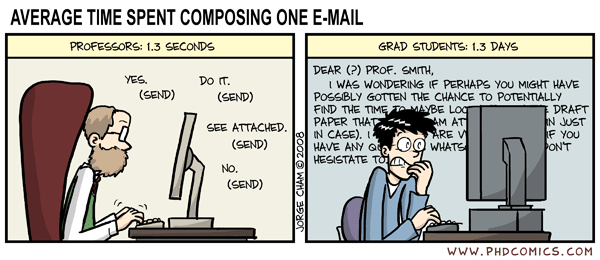
\includegraphics[scale=0.4]{files/emails.png}
\end{center}


Faculty received many "cold" e-mails from international students seeking for admission, TA, and RA. Most of the time, we ignore these emails, but in some rare occasions we do answer them. So why do we ignore some but reply to others and how to write an email that get our attention?



First, if you want to contact a prof. to \emph{ask about your admission chance}, please \textbf{don't}. We don't know and can't answer because as explained in \S\ref{sec:evalapps}, we don't make individual decisions and might not even be assigned to evaluate your application.  It is the same as sending a paper draft to a journal editor and ask them if your paper has a chance.  

So what to do if you want someone to look at your profile and give input? You could ask your professors, collaborators, or those who have previously applied. For these kind of feedback,  don't ask strangers like random profs., instead ask someone you have personal connection with.  

If you want to contact a prof. to ask about \emph{research opportunities}, or \emph{GTA/GRA} support, then \emph{yes}, I believe you should---it is \emph{worth it}. However, you need to put effort into it and really do it the \emph{right way}.



First, read the prof's website, see if they say something about contacting them. Many profs. explicitly indicate how prospective students should (or should not) contact them (e.g., using specific email subjects).
In general, the best way to catch the prof.'s attention is to \emph{customize your email} for them.  For example, read their papers, know what they work on, and see if you are interested in their research. Then send them an email talking how/why their work would match yours.
In contrast, if you write a generic email that can be sent to multiple professors (e.g., if you just change some names and keywords in the email or copy and paste paper titles), you will not get a response.

Below is a good example that I would reply to.   

\begin{commentbox}[Dear Prof. Nguyen,]

  I am writing to inquire about potential research opportunities as a GRA in your group at GMU. Currently I am an undergraduate student in Computer Science at UNIV and plan to graduate in May 2023.


  I have read your TSE'21 paper on numerical invariant generation, and I am interested in this line of dynamic invariant research. I have worked (optional: with prof. Y at Z) on static program analysis and I think it could be used to tackle the spurious issues mentioned in your paper. I have a small paper at conference/workshop C and a project on symbolic execution at Github G.

  ...

  This is a good example because it is clearly written just for me.  It shows that the student knows about my work on invariant generation and has related  background (paper C and project G).
\end{commentbox}

Finally, profs. are very busy so don't take it personally if you don't get anything from them (though I would be very surprised if such thoughtful emails get no replies!). 


\begin{commentbox}[Xiaokuan]
  Applying for Ph.D. and contacting a potential Ph.D. adviser is a classic \textbf{`why me, why you'} problem,
  similar to looking for a job in a company.
  On a high level,
  you need to show that you have done your \emph{homework}
  regarding the professor and the university,
  and clearly explain:
  1) why do you think you are a good fit in professor A's group?
  2) why do you want to be advised by professor A, not B?
  3) why do you want to apply for university X, not Y?
  If you don't want to spend time to do your homework,
  the chance of getting a reply is close to zero.
\end{commentbox}


\begin{commentbox}
    [Deepak:]
    In my view, cold emails are not welcome by most faculty members and should be avoided. However, if one is already admitted to a program in some department, by all means, send an email to the faculty you may be interested in working with, but do mention right at the beginning that you are already admitted to the program as well as several other universities. State specific areas (preferably specific topics-ML, robotics instead of AI).
\end{commentbox}

\subsubsection*{References}
\begin{itemize}
    \item \href{https://yonatanbisk.com/emailing_professors.html}{A Note about Emailing Professors} by Yonatan Bisk
\end{itemize}

\subsection{PhD in other related fields: CE, IST, Cybersecurity}\label{sec:related-fields}

In many cases you do not have to do a PhD in CS to work in your area of interested. For example, in addition to a traditional CS department, GMU has IST and Cybersecurity departments, which have faculty  with PhD in CS and work on CS topics (e.g., AI, Security, Robotics).  So it is totally possible that you still get to do CS research and publish in CS-focused venues even if you're not in a traditional CS program.  It is  common to see faculty with CS PhD in a non-CS department as well as faculty with non-CS PhD in CS department.  

However, if your intention is a PhD in CS, then you likely need to be in the CS dept \emph{and} advised by a CS faculty. In fact, if a faculty is not in CS, it is unlikely that they can be the \emph{main} adviser of a CS PhD student---they may \emph{co-advise} or be in the PhD dissertation committee, but your main adviser will need to be a tenured or tenure-track faculty in CS. If in doubt, you should check with the CS department for their requirements.  For this specific reason,  CSRankings includes only tenured or tenured track faculty who can advise CS PhD students. I also have compiled a \href{https://github.com/dynaroars/dynaroars.github.io/wiki/Viet-CS-Profs-US}{list} of Vietnamese faculty who can advise PhD students. 


\chapter{Miscs and FAQs}
\epigraph{"I want to share something with you – the three little sentences that will get you through life; number 1: Cover for me, number 2: Oh, good idea, Boss, and number 3: It was like that when I got here."}{\textsc{The Simpsons}}

\section{What can you do to increase your admission chance?}\label{sec:improve-your-chance}


\begin{center}
  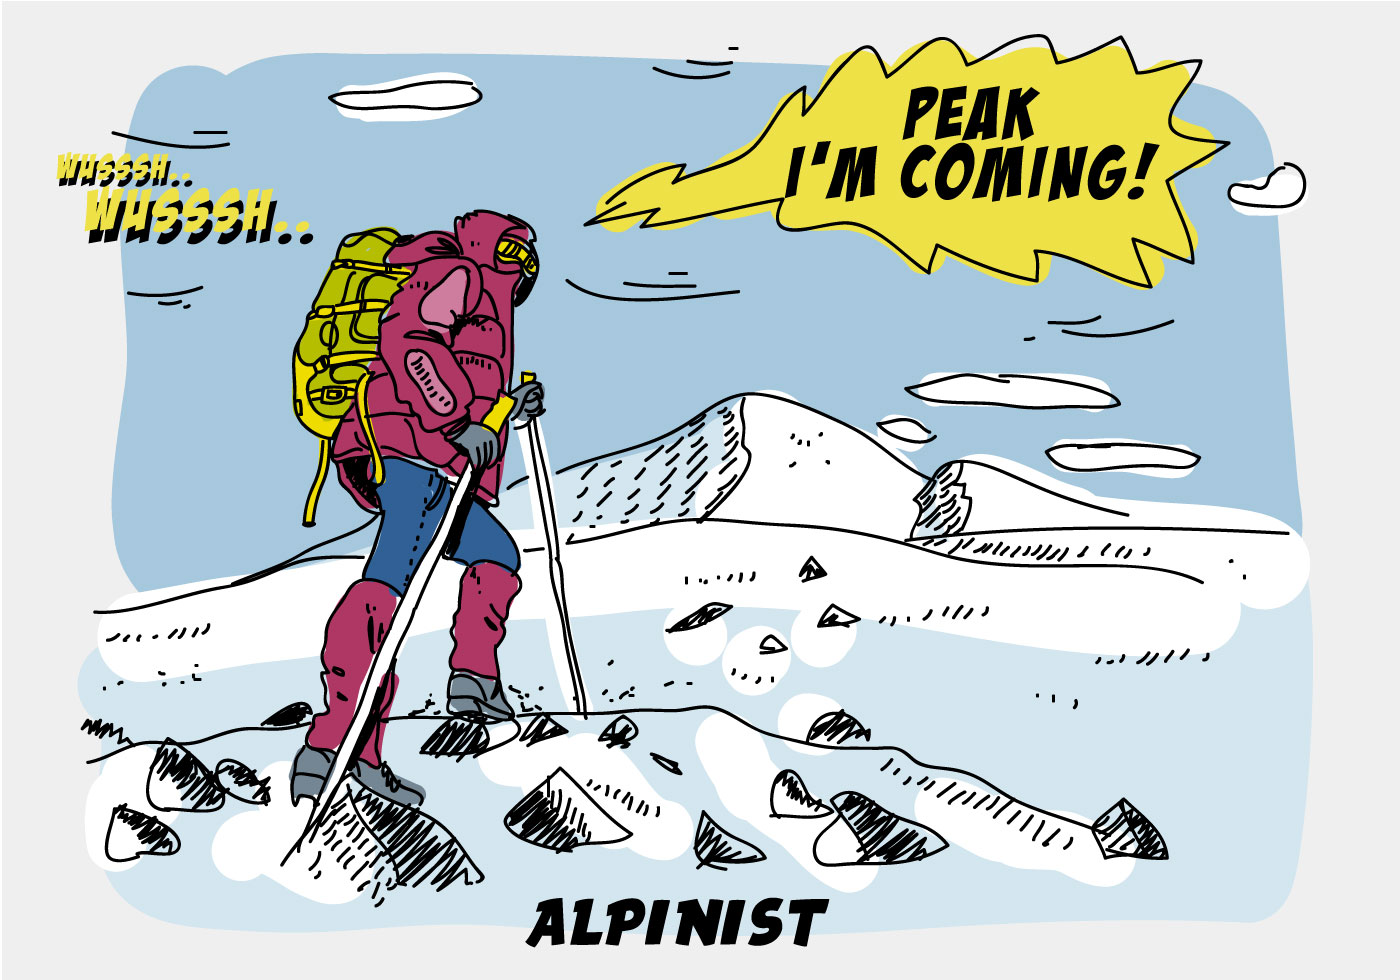
\includegraphics[scale=0.2]{files/alpinist-climbing-peak-mountain-comic-hand-drawn-vector-illustration.jpg}
\end{center}


Show something that makes you \textbf{stand out}, e.g., do you have a degree or background in \emph{dance} or \emph{music} and want to integrate them with CS? are you a female or a minority in CS (research for "URM minority in CS in the US" on Google)? Do you participate in outreach activities that help increase diversity and inclusion in CS? All of these are unique and would get noticed from reviewers.

Even if you do not have research experience, you can talk about your personal projects, as long as they can help show you can do research. For example, if you have an open-source project on Github that is used by many people, has lots of stars in Github, do talk about it. If you write technical, research-like blogs, talk about them too.


In his \href{https://matt.might.net/articles/how-to-apply-and-get-in-to-graduate-school-in-science-mathematics-engineering-or-computer-science/}{post}, Matt Might was initially unsure about an application. However, upon learning that the applicant had led a 100km hike in the Himalayas, he decided to accept the applicant.  This is a good example of being "stand out", and I would also advocate for that student as this shows they have the persistence and determination required for research.


% It is worth noting that in many cases,  an application could be rejected by most reviewers, however have a "champion", who doesn't even have to be in the Admission comittee, that strongly advocate for your profile.


\section{Can I apply to CS PhD if my undergrad was not in CS or related areas?}\label{sec:non-stem}

Yes, \emph{as long as} you can demonstrate you are ready for CS PhD research through research experiences, LoRs, statements, etc as mentioned. You might be even able to leverage this to make your profile stand out as mentioned in \S\ref{sec:improve-your-chance}. 

One main concern for non-CS or non-STEM students is if you have the sufficient technical background, typically obtained through core CS courses.  So you will want to show that you have such knowledge through your coursework, projects, or research. 
For example, if you have taken a course on Algorithms, even online ones like Coursera, you can talk about it in your statement.  If you have done a project that requires knowledge of OS or have a professional certification (e.g., A+) through work, you can talk about it in your statement.  If you have done research that requires knowledge of Discrete Maths, you can talk about it in your statement.  You can also ask your LoR writers to talk about your technical background.  
In summary, in your application, convince us that you have the technical background to do CS PhD research. 
Note that many online courses teaching about AI does not really help much as these are not core CS knowledge.

In short, you \emph{do not need} to formally taking CS courses, you just need to show that you have these essential knowledge through ways as mentioned. Many universities are well-aware that incoming graduate students might not have all the technical background, so they often have a "bridge" courses to help students catch up.  For example, GMU has four bridge courses (Data Structures and Algorithms, Computer Systems, Discrete Math, and Programming Foundation) that incoming students can take to catch up on their CS knowledge.

\begin{commentbox}[Vu:]
  I would strongly advocate for a non-STEM student who shows that they have a strong drive for CS by studying core CS knowledge through various channels (e.g., self-study through online courses, projects, etc).  I have seen many students with non-CS background who are very successful in CS PhD.  I also have seen many students with CS background who are not successful in CS PhD.  So it is not about your background, it is about your drive and passion for CS research.
\end{commentbox}

\section{Is an MS degree required for admission to PhD in CS?}\label{sec:msrequirement}
No. In fact, student with BS can get MS degree ``along the way'' to PhD.  However, MS can help if it gives research experience or is from a more well-known school than your undergrad institution. 

If you have an MS then some course work \emph{might be} transferred for course credits, which save a bit of time. But overall don't count on this, especially if your MS is not from the US. 


\section{How long does it take to complete the CS PhD program?}\label{sec:time}


\begin{center}
  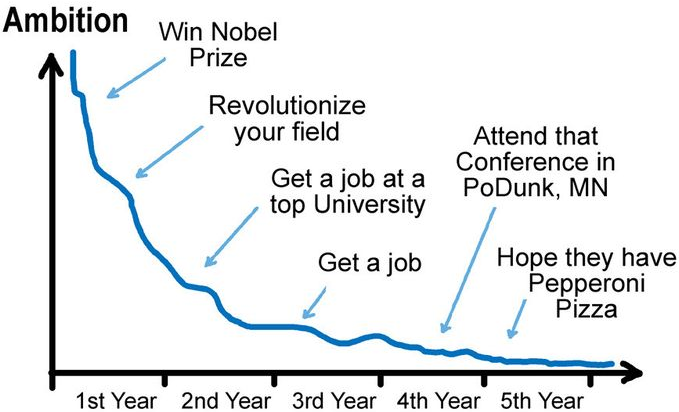
\includegraphics[scale=0.3]{files/c4a.png}
\end{center}


Typically, it takes 5--7 years for CS PhD in the US.  This can be longer than CS PhDs in other countries, which might require MS first (recall that CS PhD programs in the US do not require MS and you can get MS along the way to PhD). Within these 5--7 years, CS PhD students often take a ``leave of absence'' for 1--2 semesters to do internship at companies and research labs.

The first 2 years you typically take coursework (somewhat equivalent to an MS study), find an adviser, learn how to do research.  The next 2--3 years you focus on your research, form dissertation topic, and get results published. The last 1-2 years you continue to publish, write and defend your dissertation, and look for job.
In many cases you might take a summer or two off to do internship to get additional research opportunities.
The PhDComics figure on top shows the ``ambition'' level of a PhD student over their years of study (they miss the 6--7th year where the ambition is \emph{``Just let me graduate''}).


\section{Differences between PhD in the US and Other Countries}\label{sec:non-us-differences}

This summarizes the main differences between CS PhD in the US and other countries. % This is based on my experience and what I heard from others who did PhD in other countries. 

\emph{MS Degree requirement}:  as mentioned in \S\ref{sec:msrequirement} and \ref{sec:time}, CS PhD programs in the US do not require MS degree.  In contrast, many other countries do require MS degree before joining a PhD program.  This means that US PhD programs are longer (5--7 years, 2 of which are coursework) than other countries (3--4 years, no coursework).  

\emph{Project proposal}: in many countries, you have to choose a project and adviser \emph{during} the application process (e.g., you write a proposal to a potential adviser). In the US, you often start your PhD without an adviser or project and find them later. This is also why US PhD programs are longer.

\emph{Course work}: in the US you will spend the first couple of years taking classes and explore potential adviser and research topics. In other countries, you (who already have an MS) start your research right away, e.g., you immediately work on the research project you proposed with the adviser you chose. Also, in the US you also have to pass a series of "exams", e.g., qualifying exam, comprehensive exam, thesis proposal defense\footnote{The word "ABD" (all but dissertation) is used in the US to refer to a PhD candidate who have finished all course work and exams and only need to write and defend their dissertation.}. In other countries, you do not have to do these exams or only do a few of them.

\emph{Funding}:  In many countries stipend comes from the university or from the gov't. These funding often have a fixed duration (e.g., 3 years).  In the US, stipend (e.g., RA) comes directly from your adviser (no fixed duration).  There are also fewer TA opportunities in the European universities compared to the US.

\emph{Faculty position after PhD}: In other countries, PhD graduates who are interested academia typically apply for research positions at research labs, i.e., postdocs, and then consider faculty position. In the US, PhD graduates often apply directly for faculty position (postdoc for US graduates is no longer a popular option as it was before).  This is why US PhD programs are longer and more focused on research.

\emph{Work-life balance}: PhD students in the US are often said to be overworked compared to other countries, e.g., in Europe.  This is partly due to the longer PhD program and that US PhD students are often paid through TA, which requires them to do TA in addition to their own research. In contrast, PhD students in other countries are often paid through fellowships, which do not require them to do TA.

\section{How do I call or address a professor?}\label{sec:address}

\begin{center}
  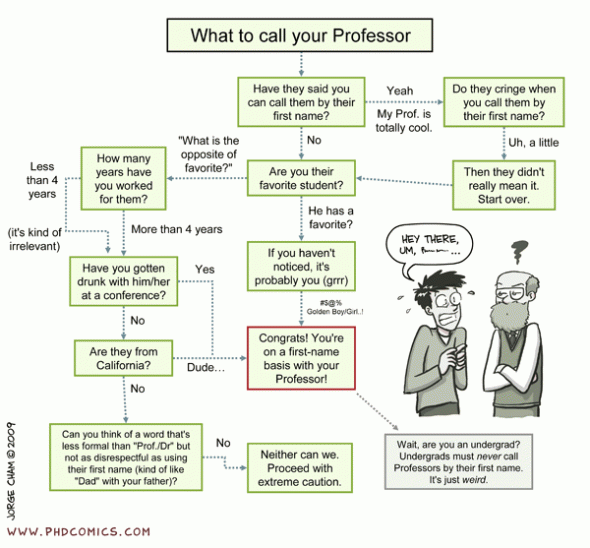
\includegraphics[scale=0.5]{files/c5.png}
\end{center}

If you're reaching out to a professor for the first time,  address them as Prof. or Dr. Lastname. Many international students use Prof. or Dr. FirstName LastName, but this can come across as if you're simply copying and pasting names. It's not necessary, so stick with Prof. or Dr. Lastname.


Furthermore, avoid using Mr. or Mrs., or the professor's first name if you're not acquainted with them yet.  As you become more familiar with your prof and depending on their preferences, you may transition to addressing them by their first name.
For example, I prefer that my students and colleague call me Vu. Some students call me \emph{Dr. Vu}, which I find a bit amusing but am totally fine with it. 

\begin{commentbox}[DK:]
  I was amused to read this as if I recall correctly, you never called me by my first name when you were at UNM. You always called me Prof. And, many times, I would jokingly call you back as Prof. Vu.
  \tcblower
  \textbf{Vu}: Yes, for some reason I enjoy addressing you as ``Prof.'' (without appending a last or first name).  The use of Prof. Vu may have foreshadowed my future in academia.
\end{commentbox}

Note that in some universities the formal title Dr. Lastname is preferred over Prof. You just need to observe and follow the conventions at your particular institution. Additionally, be aware that not all faculty members may hold a Ph.D., in which case using Prof. Lastname is a suitable alternative.


\paragraph{Referring to professors you know} Because you are already familiar with these individuals, you can just informally use their names if they are OK with it as mentioned above (or Dr./Prof., if you want to be formal). You can also include their institution if it makes it more precise.  For example, I can say:  \emph{"I did my postdoc with Jeff Foster at Univ. of Maryland"}.   

Do not include ranking (e.g., Assistant, Associate, Scientist, ...) when referring to someone. I see many international students include a lengthy title of people they know, e.g., \emph{I am advised by Asst. Prof. X, and I also collaborate with Distinguished Scientist Y}.  This is \emph{not necessary} and makes it look like you're trying to show off your connections. These nuances represent some cultural differences that you may encounter and will gradually adapt to. More on cultural differences in \S\ref{sec:cultural}.

\section{How much do \emph{you} cost?}\label{sec:ra-cost}
PhD students often ask why their salary is so low compared to ludicrous grants their advisers get. They also wonder why their offer letters sometimes show that their benefits higher than what they actually receive (i.e., stipend).  This section aims to shed some light to these questions.

\begin{center}
  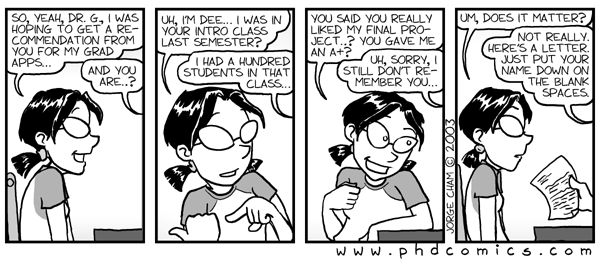
\includegraphics[scale=0.3]{files/c6.png}
\end{center}

\begin{table}
  \centering
  \small
  \caption{GRA cost breakdown. F \& A is Facilities \& Administrative Cost Base and
    MTDC is Modified Total Direct Cost. These are things that the university can charge overhead to.}\label{tab:cost}
  \begin{tabular}{rcl}
    \textbf{Budget} & \textbf{Cost \$} & \textbf{Notes} \\
    \midrule
    GRA (9-month) & 27K & \\
    GRA (summer)  &9K	& 3-month, 20hrs/week\\
    \textbf{Total Salary} &\red{36K}	&\\
    \midrule
    Health Insurance	&3K	& full year\\
    Tuition (In-State) &	15K	& (\$680/ Credit + \$150/Student Fee/ Credit)* 9 credits = \\
                    &&\$7470 (\$6120 + \$1350) per semester\\
    \textbf{Total Tuition \& Insurance}	&\red{18K}	&Full year tuition + insurance\\
    \midrule
    Conference Registration	& 500 & \\
    International Travel &	1800& \\
    Domestic Travel	& 700	& \\
    \textbf{Total Travel}&	\red{3K}	\\
    \midrule
    Total Direct Cost	& \red{57K}	&Salary + Travel + Health + Tuition \\
    F \& A (MTDC)	& 21K	& Direct Cost - GRA Salary\\
    Total Indirect Cost	& \red{12K}	&58.9\% of MTDC\\
    \textbf{Total (Direct + Indirect)} &	\red{69K}	& Budget for a GRA\\
    \bottomrule
  \end{tabular}
\end{table}

Tab.~\ref{tab:cost} shows the budget breakdown for a GRA per year (this level of details is what faculty actually uses when applying for grants).
These numbers are based on my experience at public universities in the US.  Private universities may have different numbers.  For simplicity, in this table I will assume the department has a 9-month stipend of \$27000 (GMU actually pays more) and therefore a 3-month summer of \$9000. I will also use GMU tuition rate of about \$15,000/year for full-time study (which is quite cheap compared to private universities, e.g., MIT charges around \$50K) and a 58.9\% rate on \emph{indirect cost}, which is what GMU charges for overhead or administrative costs (yes, after all, universities are businesses!).  Finally, I assume the student take two conference trips per year, one domestic and one international (conf. registration, airline tickets, taxi, meals, etc are all included). 

At the end, the total budget comes out to be \$69K/year to support a PhD student. \emph{The summary is that over your 5-6 year of your PhD, you cost about \$350K--400K, and while you're paid X, your adviser probably pays 2X for you}.  


% \section{Having fun during a PhD?}
% PhD students \emph{and faculty} probably find it amusing about the notion that students, especially international ones, can genuinely enjoy their PhD studies. In fact, after reading posts after posts on VietPhD.org on how PhD students are commonly mistreated, stressed, it seems being miserable is a norm during a PhD study.

% There are many advice on surviving PhD that you can follow. But here I just list a few that works for me and what I advice my students to do.\tvn{TODO}


\section{Will I be miserable during my a PhD?}\label{sec:happy}
There are many stories on how students are mistreated, stressed, and miserable. Certainly issues including bad relationships with professors, conflicts with co-authors and lab mates, and toxic working environment, feeling left out or discriminated (e.g., because you're an international student) \emph{do} exist, and it is good to be aware of those.  However, in reality there are many good mentors, supportive lab mates and department, happy students, etc.  So don't let social media make you feel pessimistic and deter your quest to advance knowledge.

\chapter{Cultural Differences and Other Issues}\label{sec:cultural}

This section lists various cultural issues that international students might want to pay attention to.

% \paragraph{Diversity} US universities prioritize diversity and inclusion. Students need to respect and appreciate varied opinions, backgrounds, and cultures. Unlike some countries where certain voices are marginalized, in the US, all perspectives are valued equally (especially at universities). Racism or discrimination will have serious consequences, including academic and disciplinary actions.

\section{Academic Integrity} 

Plagiarism and cheating (e.g., exams, assignments) is a BIG no-no in the US.  If you're caught cheating, you will face very heavy consequence and likely be expelled from the university (e.g., after the second time at GMU).   This is quite different from many international countries where cheating is common and often tolerated.  Faculty is extremely good at detecting cheating (we have been dealing with these situations so many times over so many years), and \emph{will} report cheating cases.  In short, whatever you do, don't cheat---not worth it.

Here is the typically steps: (i) a faculty suspecting a cheating case will report it to the Office of Academic Integrity (OAI) at the university---the report often has supporting evidence and suggested penalty (e.g., a failing grade);  (ii)  OAI will take over and investigate the case; and (iii) OAI will make the final decision.  It is important to note that after receiving the report from your prof., OAI \emph{completely} takes over and makes decision.  This means begging your professor will not help because they simply are no longer involved in the case.

\section{Illegal Software} Using illegal/cracked software is very common in many countries (and even in the US). However, \emph{do not} install or use them on university computers (e.g., those given by your department or adviser).  It is unlikely that the university will track you down, but it is the \emph{software company} that will.  They have very sophisticated tools to detect illegal software and will sue your university/department.  Imagine your department or adviser being sued for a large sum of money, and it is \emph{you} who caused it.  If you need software, ask your adviser or the department.


\section{Gifts} In many countries, it is customary to give professors gifts, often during holidays.  These gifts can be costly and profs. sometimes expected them. In the US, it is uncommon and perfectly OK to not to give gifts. \emph{However}, if you'd like to offer small souvenir-like tokens, it's a thoughtful gesture that's appreciated. Some professors proudly display their gifts, which can come from students and colleagues (e.g., when they travel to their home countries or conferences). In summary, small gifts are fine, but avoid anything that might make your professors uncomfortable.


There's a misconception that in the US it's all business, with professors as bosses who pay students for their work, and you doing something nice implying you expect something in return. However, the reality is quite the opposite. While people can be straightforward and direct, they are also friendly and informal. You can call your professor by their first name (\S\ref{sec:address}), disagree with them and argue (and gain respect doing so), seek their help (even on personal matters), come to their houses for parties or gathering, and give them small thoughtful gifts that they put on their desks.  Many students and professors maintain lifelong relationships, staying in touch through cards, emails, and calls, even after their academic journey ends.% These connections are genuine and meaningful.

% \begin{commentbox}
%     [DK:] Here are a few items you may consider addressing: putting international students in touch with other students from their countries, assuring them that they would be picked up from airports upon their arrival and that their initial stay will be taken care of. Most universities have other resources for these, but it is worth mentioning that they would be taken care of upon arrival and can get help during the transition phase. Learning to cook was a big deal when I arrived over 50 years ago-August 1973. But things have changed as one can find many ethnic food places, a big contrast from 1973, when there were two Indian restaurants in Greater Boston area.
% \end{commentbox}





\appendix

\chapter{Ranking of CS PhD programs}\label{sec:ranking}


\begin{table}
  \centering
  \small
  \caption{Top 50 CS PhD programs in the U.S. (CSRankings, June 2023). \red{$^*$} indicates that the university has \href{https://github.com/dynaroars/dynaroars.github.io/wiki/Viet-CS-Profs-US}{Vietnamese prof.} that can advise CS PhD students.}\label{tab:ranking}
  \begin{tabular}{rl|rl}
    \toprule
    1 & Carnegie Mellon & 26 & Univ. of California - Irvine \\
    2 & Univ. of Illinois at Urbana-Champaign\red{$^*$}  & 27 &  Duke University \\
    3 & Univ. of California-San Diego & 28 & Rutgers University\red{$^*$} \\
    4 & MIT & 29 & Univ. of California - Riverside\\
    5 & Georgia Institute of Technology         & 30 & Northwestern University\\
    6 & Stanford University& 31 & Pennsylvania State University  \\
    7 & University of Michigan - Ann Arbor\red{$^*$}   & 32& George Mason University\red{$^*$}\\  
    8 & University of Washington      &33 &  Harvard University \\
    9 &  Univ. of California - Berkeley  &34&  Univ. of California - Santa Cruz \\
    10 & Cornell University  & 35 &  Yale University \\
    11 & University of Maryland - College Park &  36& Brown University \\ 
    12 & Northeastern University\red{$^*$} &37&  Ohio State University\\
    13 & University of Wisconsin - Madison\red{$^*$}  &38& Texas A\&M University\red{$^*$} \\
    14 & Columbia University   &39 & Boston University  \\
    15 &   Purdue University  &40& North Carolina State University\\\  
    16 & University of Texas at Austin   &41 & University of Utah \\
    17 & University of Pennsylvania\red{$^*$} &42 & University at Buffalo\red{$^*$}\\
    18 & Princeton University  & 43& Rice University\\
    19 & University of Massachusetts-Amherst\red{$^*$} & 44&  University of Colorado-Boulder \\
    20 &  New York University  &45& University of Illinois at Chicago  \\
    21 & Univ. of California - Los Angeles &46& Virginia Tech\red{$^*$}  \\
    22 & University of Southern California &47&  Arizona State University\red{$^*$} \\
    23 & Stony Brook University\red{$^*$} &48&University of Minnesota \\
    24 & University of Chicago &49& University of Virginia \\
    25 & Univ. of California - Santa Barbara &50& University of North Carolina\red{$^*$} \\
    \bottomrule
  \end{tabular}
\end{table}

Tab.~\ref{tab:ranking} lists the top 50 CS programs in the US from \href{https://www.csrankings.org}{CSRankings.org}, a ranking system  based on top CS conferences.

% \section{Additional Resources}
% \begin{itemize}
          %     \item \bibentry{nlpphd}
          %   \end{itemize}

%\chapter{References}


\chapter{History and Acknowledgement}\label{sec:ack}

\paragraph{History} This document was conceived during a lunch with Craig Yu at GMU.  We talked on about why GMU were not able to attract good Vietnamese and other international students, despite having a much stronger CS program than many schools that these students want to go to (part of the reason is described in \S\ref{sec:selecting-ranking-schools}). We wished there were a way for international students to know about the US PhD programs (as well as for US faculty to understand more about international students and therefore have better chance of recruiting and working with them). I was also  a member of the large VietPhD group on Facebook and saw many questions from students about PhD programs.  However, most active participant are students in non-CS fields or not in US. Like ChatGPT, their answers to questions on CS PhD program in the US could be informative and helpful, but unfortunately not always accurate and sometimes leading to more confusion. So I thought it would be useful to have a document that is specific to CS PhD programs in the US from an insider prospective.

I started writing this document in May 2023 and have been updating it since then (mostly around deadline time when I tend to procrastinate, i.e., \emph{productive procrastination}!). I have put the source code of this document on \href{https://github.com/nguyenthanhvuh/phd-cs-us}{GitHub} so that anyone can contribute to it.  

\paragraph{About Me} I am an assistant professor in the CS dept at George Mason University (GMU). Prior to GMU, I was at the University of Nebraska-Lincoln (UNL). I have been in the PhD admission process at GMU and UNL for many years.  Currently I serve as the program director of the MS program in Software Engineering at GMU (thus also have some experience with the MS admission process--which is quite different than PhD). %I got my undergraduate and MS degrees from Penn State. I completed my PhD at the University of New Mexico-Albuquerque and a postdoc at the University of Maryland-College Park.

While I am not an international student, many of my students and collaborators are.  I also mentor multiple students from Vietnan, and have various colleague and friends who were international students. I have heard their stories, and hope to capture their challenges and experiences in this document so that it can be useful for prospective international students.

\paragraph{Acknowledgement} Many people have contributed to this document.
Profs. Craig Yu (GMU), Hakan Aydin (GMU), 
Xiaokuan Zhang (GMU), Hung Le (UMass), and Deepak Kapur (UNM) provided valuable input in the early version. Other GMU faculty members also have provided feedback and contributions.  Many students including Didier (GMU), Thanh (Melbourne), and Dat (Melbourne) have contributed valuable questions and feedback.
\textbf{Thank you!}



\bibliographystyle{abbrv}
\bibliography{demystify.bib}

          %           \newpage
          %           \section{Virtual Research Opportunities Beyond Physical Boundaries (written by Didier)}
          %           \didi{In my experience, prospective PhD students (from Rwanda) are often unaware of the information provided in this document throughout their undergraduate. For this reason they often find themselves unprepared for PhD admission process by the time they finish undergraduate and have to spend a year or more to improve their application profiles. I think it would be beneficial to expand the document to also target students who are not yet ready for the application process to help them improve on all criteria considered during admission. I drafted the short essay on how to gain research experience remotely in order to improve their research profile and potentially get LOR from experts (hopefully faculty)}\\
          %           In the realm of computer science, research experience plays a crucial role in securing admissions to top-tier Ph.D. programs. However, students from underrepresented small colleges, both in the United States and internationally, often encounter limited research opportunities within their institutions. Thankfully, there exists an alternative pathway for these aspiring researchers to gain valuable research experience, even without being physically present at a university.

          %           \textbf{Virtual Research Programs}:
          %           Several universities, organizations, and research institutions offer virtual internships and research programs aimed at providing hands-on research experience. These programs often involve working remotely under the guidance of experienced mentors and collaborating with a team of fellow researchers. For instance, \href{https://docs.google.com/forms/d/1btIwt4HwjyKMOUk-EMy3rbkfWzFxv2lNrMm_zkd0pA4/viewform?edit_requested=true}{UIUC+ Summer Undergraduate Research in Software Engineering}  offers an unpaid remote internship for software engineering students all over the world to collaborate with mentors from University of Illinois at Urbana Champaign.
          %           Virtual internships offer opportunities to contribute to ongoing research projects, conduct experiments, analyze data, and write research reports. Students can search for such programs through university websites, research institutes, or as of recently chatGPT (or Bard).

          %           \textbf{Online Research Communities and Open Source Contributions}:
          %           Online research communities and platforms offer a wealth of opportunities for aspiring researchers. Platforms like GitHub, GitLab, and Bitbucket host repositories spanning diverse research domains. Students can explore repositories related to their areas of interest, collaborate with other contributors, and actively engage in open source research projects. By contributing code, fixing bugs, implementing new features, or providing documentation, students can gain practical research experience and interact with experienced developers and researchers in the field.

          %           \textbf{Online Conferences and Workshops}:
          %           Attending online conferences and workshops is another way to gain exposure to cutting-edge research and establish connections with experts in the field. Many conferences now provide virtual participation options, enabling students to access research talks, poster sessions, and panel discussions and sometimes access designated chat rooms or networking events where participants can engage with researchers, ask questions, and seek potential research collaborations. It is beneficial to also create profiles academic collaboration platforms such as ResearchGate. By creating profiles, joining relevant research groups, and participating in discussions, students can connect with established researchers, contribute to ongoing projects, and potentially collaborate on publications or research proposals as they provide access

          %           In conclusion, for students lacking research opportunities at their small colleges, the virtual realm offers a wealth of possibilities to gain valuable research experience. Engaging with open source projects, joining online research communities, utilizing academic collaboration platforms, participating in virtual internships, and attending online conferences are all avenues to contribute to research, connect with experts, and enhance one's research profile.


\end{document}

